\chapter{Analysis of Evolutionary Breakpoint Features}
\label{chap_breakpoint_analysis}

This chapter describes a data analysis project unrelated to the algorithmic development of Cloudbreak and its extensions, although it is related at the biological level because it deals with genome breakpoints and rearrangements. In addition to being able to locate genomic breakpoints, we also seek to understand the genomic contexts in which they are located to gain insights into their origins. As we discussed in Chapter~\ref{chap_background}, the sequence features of the genome that neighbor structural variations can leave clues about the mechanisms that caused the rearrangements, as in the cases of large homologies that point to the activity of non-allelic homologous recombination (NAHR) or the microhomologies that indicate non-homologous end joining (NEHJ). In this chapter we examine a set of structural variations that have reshaped a genome at the evolutionary timescale: the chromosomal rearrangements of the gibbon genome. We analyze the locations in which the gibbon genome has been rearranged relative to humans and the other apes, first using a smaller set of breakpoint data, and then using the entire gibbon genome reference sequence created by the International Consortium for Sequencing and Annotation of the Gibbon Genome. The associations we discover could help to provide insights into the mechanisms into which the gibbon genome was rearranged. \todo{and perhaps its structure and function} The main contributions of this chapter are 1) the statistical analysis of the enrichment or depletion of certain genomic features in regions of the gibbon genome that have participated in genomic breakpoints, 2) development of an open-source software tool that can harness compute clusters to conduct permutation analysis for statistical enrichment of features in the genome, and 3) a novel, cross-species analysis of the locations of binding sites of the transcription factor CTCF with respect to genome breakpoints in the gibbon family.

\section{Background}

In Chapter~\ref{chap_background}, we described how SVs can occur in the genomes at many different levels, ranging from the rearrangements that occur in populations of cells within a tumor in a single individual, to SVs that are polymorphic within the population of a species, and all the way to the structural differences between the genomes of different species. This last type of rearrangement represents SVs that occurred within a population and then became fixed in that species and were preserved as it evolved and differentiated. 

Rather than identifying them by comparing short-read sequencing data to a reference genome, as has been the focus of the previous chapters, we can detect these evolutionary breakpoints by directly comparing the genomes of species to each other. This can be done biochemically, by mapping the location of individual genes or large fragments of DNA from one species to particular chromosomes in another; this is the case of the BAC analysis we will describe in Section~\ref{gibbon_breakpoint_bac_analysis}. With the advent of whole genome sequences they can be found by conducting sequence alignments (or multiple sequence alignments) of the the reference genomes for the species under study. When species share regions that contain the same genes and other genomic features, in the same order, it is referred to as \emph{shared synteny}. By examining the endpoints of syntenic blocks of the genomes of two species, or \emph{synteny breakpoints}, it is possible to find the breakpoints of the structural variations that rearranged the structure of the two genomes.

Identifying evolutionary breakpoints can give insights into the mechanisms of their formation. It was long thought that chromosomal breakpoints were largely random, such that they are equally likely to occur at any location in the genome~\cite{Ono:1973tr,Nadeau:1984tm}. Higher-resolution analysis, however, revealed that certain regions of the genome are much more likely to give rise to evolutionary breakpoints~\cite{Pevzner:2003ba}, and this result was re-confirmed once whole-genome reference sequences for many species became available~\cite{Murphy:2005hv}. Tantalizingly, Murphy et al. also showed that these reused evolutionary breakpoint regions overlapped significantly with the breakpoints of SVs found in cancer genomes~\cite{Murphy:2005hv}.

This raises the question of whether these regions of the genome have special properties that make them more likely to participate in evolutionary breakpoints. In Chapter~\ref{chap_background}, we described the fact that certain mechanisms for SV formation, in particular NAHR, are a result of having regions with high sequence similarity at different locations in the genome, as the cell's machinery attempts to repair double-stranded breaks in DNA by joining homologous regions together. As one might expect if evolutionary breakpoints were the result of NAHR, a large number of chromosomal rearrangements in mammals, approaching 40\%, are associated with segmental duplications~\cite{Bailey:2004fb,Bailey:2006fn}. Closer examination of breakpoints from a variety of species, including human, chimp, macaque, rat, mouse, pig, cattle, dog, opossum, and chicken, confirmed that they contain more sequence that is not unique relative to the rest of the genome than would be expected by chance, including segmental duplications (SDs) and other low-copy number repeats~\cite{Larkin:2009ij}. However, analysis of evolutionary sequence divergence in these repeats indicates that some of the duplications may have occurred after the rearrangements, casting doubt on the theory that an NAHR-like process is primarily responsible~\cite{Bailey:2004fb}, and indeed the precise mechanisms behind evolutionary breakpoints remain unknown.

Gibbons represent a unique opportunity to study the process of evolutionary genomic rearrangement because of their highly rearranged genomes. In most branches of the evolutionary tree, large genomic rearrangements are rare events, occurring at a rate of approximately two every ten million years~\cite{Wienberg:2004gt}. However, some species appear to have faster or slower rates of rearrangements. For example, the orang-utan genome has very few medium and large scale rearrangements relative to the expected number given its time of evolutionary divergence~\cite{Locke:2011gn}. At the other end of the spectrum, gibbon genomes have 10 to 20 times more rearrangements than would be expected given the rate in other mammals, and in fact the four genera of gibbons have numbers of chromosomes ranging from 28 to 52, suggesting that gibbon genome has been shuffled rapidly since it diverged from the other apes 17 to 18 million years ago~\cite{Misceo:2008kg}.

Given their highly rearranged karyotypes, gibbons represent an excellent model in which to study mechanisms of chromosomal rearrangements. Until recently, however, the whole genome sequence of the gibbon was not available. Therefore, several studies analyzed gibbon genome breakpoints using techniques involving bacterial artificial chromosomes (BACs)~~\cite{Girirajan:2009kw,Carbone:2006jk,Carbone:2009p1012}. BACs are medium sized (150-350kb) fragments of DNA from a sample that are isolated, turned into plasmid bacterial chromosomes, and then amplified in a culture. By probing gibbon BACs with arrays or testing their hybridization to human chromosomes using fluorescent \emph{in situ} hybridization (FISH) experiments, it is possible to isolate BACs which span human-gibbon evolutionary breakpoints. This allows one to locate the breakpoint regions to within several hundred kilobases, and the small size of the BACs relative to the entire genome makes them much easier to sequence, allowing the analysis of sequence features near the breakpoints; or, if sequencing is not possible, to identify the regions orthologous to the breakpoints in the genome of a well characterized genome. Initial studies examined selected BACs from the northern white-cheeked gibbon species \emph{Nomascus leucogenys leucogenys} (NLE) and found a high level of segmental duplications and repetitive sequence at the breakpoints~\cite{Carbone:2006jk,Roberto:2007dt}. Similar results were found in BACs from the white-handed gibbon species \emph{Hylobates lar} (HLE)~\cite{Misceo:2008kg}. A later study increased the scope by examining 24 sequenced NLE BACs that spanned breakpoints, and analyzed gibbon-specific insertions of repeats and segmental duplications at the breakpoints to postulate several possible rearrangement mechanisms~\cite{Girirajan:2009kw}. More recently, Carbone et al.~\cite{Carbone:2009p1012} analyzed 57 NLE BACs and, in addition to segmental duplications, found enrichment for \emph{Alu} repetitive elements. The latter study also found differences in CpG methylation marks on \emph{Alu} elements near the breakpoints, suggesting that there may be an epigenetic process involved in gibbon genomic rearrangements.

\section{Evolutionary Breakpoints in the Gibbon Genome  Identified by BACs}\label{gibbon_breakpoint_bac_analysis}

To determine whether or not the characteristics observed in the breakpoints identified by BACs from NLE and HLE gibbons were generalizable to the entire gibbon family, we conducted an expanded analysis of gibbon breakpoints based on the identification of additional BACs covering breakpoints in the remaining two gibbon genera using samples from the species \emph{Symphalangus syndactylus} (SSY) and \emph{Hoolock leuconedys}. Since each of the gibbon genera has a different karyotype, identifying breakpoints across all four allows for greater insight into the mechanisms and timing of the evolution of the gibbon family. I contributed to this research by analyzing the overlap between breakpoints from all four gibbon genera with genomic features. This work was published in Capozzi et al.~\cite{Capozzi:2012bb}.

\subsection{Methods}

To determine whether there exists an enrichment or depletion for genomic features associated with gibbon chromosomal breakpoints we computed the significance of their overlap using Monte Carlo permutation tests. The purpose of the permutation analysis is to discover the null distribution for the number of overlaps a set of intervals has with a particular feature in the genome. In essence, the test asks: if my intervals were placed in random locations on the genome, what is the probability of seeing the number of overlaps we observed with that features in the actual data? In this case, the intervals whose locations we permute are the gibbon breakpoint regions.

For this test, we identified the human regions that are syntenic to the locations of the breakpoints in gibbons. We then permuted their start coordinates 10,000 times using BEDTools version 2.16.2~\cite{Quinlan:2010km}, while maintaining the chromosomal assignment and length of breakpoint regions. Genomic regions annotated as centromeres and telomeres in the ``Gaps'' track of the hg19 build were excluded from possible random placements of the regions. Locations of the features were held constant. We then compared the actual number of features that overlapped a breakpoint region to the distribution of overlap counts among the randomly permuted regions, and used the quantile of the real observed value in that distribution as an estimate of the P-value of observing a value equal to or greater than the real observation. For events that are rare, it is necessary to consider a large number of permutations or Monte Carlo samples in order to accurately estimate the p-value~\cite{Rubinstein:2007:SMC:1349778}. In order to facilitate conducting many permutations, we created a pipeline for distributing the necessary computation across a compute cluster using the grid management system HTCondor~\cite{condor-practice}.

The analysis was performed on the human hg19 assembly. The features examined were genes, human segmental duplications, and some repeat families (\emph{Alu}, LINE, ERV, and SVA). We also investigated the associations between breakpoint regions and chromatin structure by testing the overlap with open chromatin regions in human embryonic stem cells reported by the ENCODE consortium~\cite{ENCODEProjectConsortium:2011iz}. 

\subsection{Results}

We found a significant enrichment for genes (Bonferroni adjusted P-value = 0.0287), human segmental duplications (P = 0.0366), \emph{Alu} (P < 0.0001), and SVA (P = 0.0008) Figure~\ref{gibbon_bac_permutations} displays the histograms of overlap counts in the random distributions for segmental duplications, \emph{Alu} elements, and SVA elements. We did not find significant enrichment for LINE and ERV repeats, nor for the ENCODE open chromatin regions. SVA elements are not found in gibbons; therefore, their status as significantly enriched in the human syntenic breakpoint regions is surprising. However, SVAs are known to correlate with \emph{Alu} elements due to their preference for G+C rich regions of the genome (Wang et al. 2005). It seems likely that the association between human SVA locations and gibbon breakpoint regions is therefore an indirect one, dependent on the presence of additional genomic features present in both humans and gibbons. 

Systematically shifting the location of breakpoint regions by increments of 10 kb up- and downstream of their actual location, up to a maximum of 1 MB, shows that the locations of the breakpoint regions gives the greatest or close to the greatest number of overlaps with the four significantly overlapping features (genes, segmental duplications, \emph{Alu}, and SVA) in the local genomic neighborhood, also shown in Figure~\ref{gibbon_bac_permutations}.

\begin{figure}
\centering
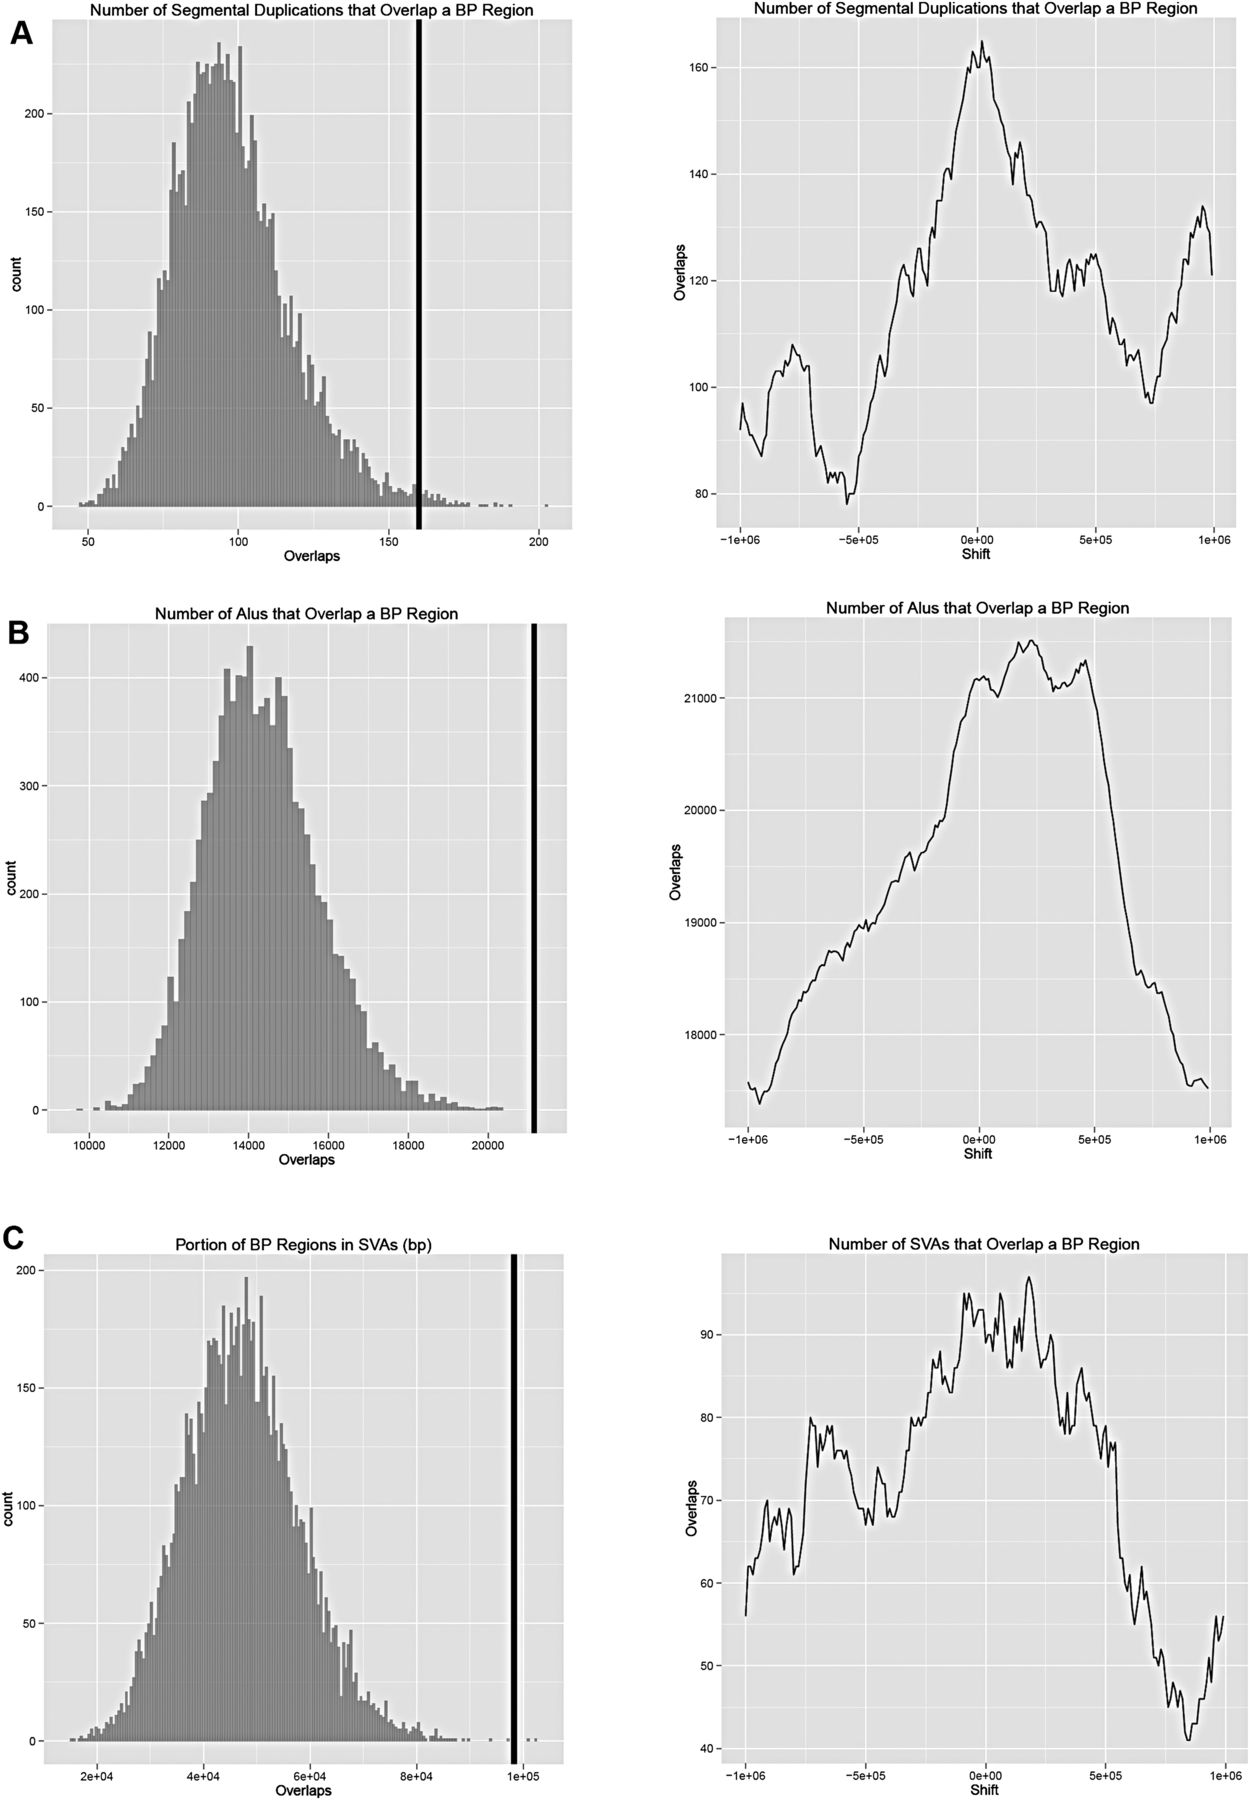
\includegraphics[width=.85\textwidth]{figures/gibbon_bac_permutations.jpg}
\caption{Enrichment of genomic features in regions of the human genome syntenic to gibbon breakpoint regions identified using BACs. Permutation tests were used to assess the overlap between the gibbon breakpoints and genomic features. (A) Segmental duplications; (B) \emph{Alu} elements; and (C) SVA elements. The black vertical line indicates the observed value for the breakpoints identified in the study. In all three cases it is evident that the genomic features have a higher overlap with the breakpoints than one could expect by chance. Figure reproduced from Capozzi et al.~\cite{Capozzi:2012bb}.}
\label{gibbon_bac_permutations}
\end{figure}

\section{Analysis of Breakpoints from the Gibbon Genome Reference Sequence}

While analysis using breakpoints identified with BAC clones has provided useful results, the International Consortium for Sequencing and Annotation of the Gibbon Genome has recently created a draft assembly of the whole gibbon genome for an NLE individual. Comparison of the assembly sequence with the human reference genome has enabled the identification of a complete set of synteny breakpoints between the human and gibbon genomes at single nucleotide resolution. This allows for a much more comprehensive picture of the sequence features surrounding gibbon breakpoints than was previously possible. As a member of the project, I was responsible for the breakpoint analyses described here.

\subsection{Overlap with Genomic Features: Repeats and Genes}

To analyze the enrichment of genomic features in the regions flanking evolutionary breakpoints, we again used a permutation based approach. The number of overlaps between breakpoint flanks and each feature of interest in the assembled genome (the observed overlap count) was again compared to a background distribution estimated by randomly permuting the locations of breakpoint regions 100,000 times. The Nleu1.1 version of the assembly was used for these analyses. To create breakpoint regions, for those breakpoints for which we had single nucleotide resolution we added flanking regions to either side of the breakpoint; for breakpoints that fell within a gibbon-specific repeat element, we chose the flanking regions of the repeat. In each permutation, the location of each breakpoint region was randomly changed, while keeping the length and scaffold assignment of the breakpoint region the same. We then counted the number of overlaps between the randomized breakpoint regions and the feature of interest (the permuted overlap count). Enrichment p-values were computed as the proportion of permuted overlap counts that were more extreme than the observed overlap count. We also visualized the spatial relationship of breakpoint regions to each type of figure by simultaneously shifting the locations of the breakpoint regions up to 1MB in each direction, in increments of 25kb, and counting the proportion of shifted breakpoint regions that overlapped a feature of interest, after discarding regions that were shifted beyond the beginning or end of a scaffold. Permutation testing and shift testing were carried out using custom Python scripts and the BEDtools~\cite{Quinlan:2010km}, pybedtools\cite{Dale:2011cl}, and BEDOPS~\cite{Neph:2012kq} libraries. For this project we enhanced the pipeline and made the code publicly available at \url{https://github.com/cwhelan/permuting-feature-enrichment-test}.

We tested for enrichment in the breakpoint regions of the following features: genes, segmental duplications, and several classes of repetitive elements: \emph{Alu}, L1, LAVA, and LTR. In addition to testing the entire \emph{Alu} family, we also tested the subfamilies \emph{AluS}, \emph{AluJ}, and \emph{AluY} individually. Gene locations were taken from Ensembl build 70. For the segmental duplication analysis, we used the segmental duplications identified by our collaborators in the Eichler laboratory using the WSSD method~\cite{Bailey:2002jp}. \emph{Alu}, L1, and LTR locations were identified using RepeatMasker output. In order to determine the distance from the breakpoints at which enrichments are strongest, we varied the size of the breakpoint flanking regions by adding differently sized intervals; we tested flanking regions of size 100bp, 250bp, 500bp, and 1000bp. We corrected for multiple testing using the FDR under dependency method of Bejamini and Yekutieli~\cite{Benjamini:2001fs}. 

Breakpoint regions are depleted for genes, but enriched for \emph{Alu} elements and segmental duplications. The enrichment for \emph{Alu} becomes particularly strong at distances of 750bp or 1000bp from the breakpoint (Figure~\ref{gibbon_genome_enrich_by_distance}). The enrichment for \emph{Alu} is primarily due to a strong enrichment of the \emph{AluS} subfamily.

\begin{figure}
\centering
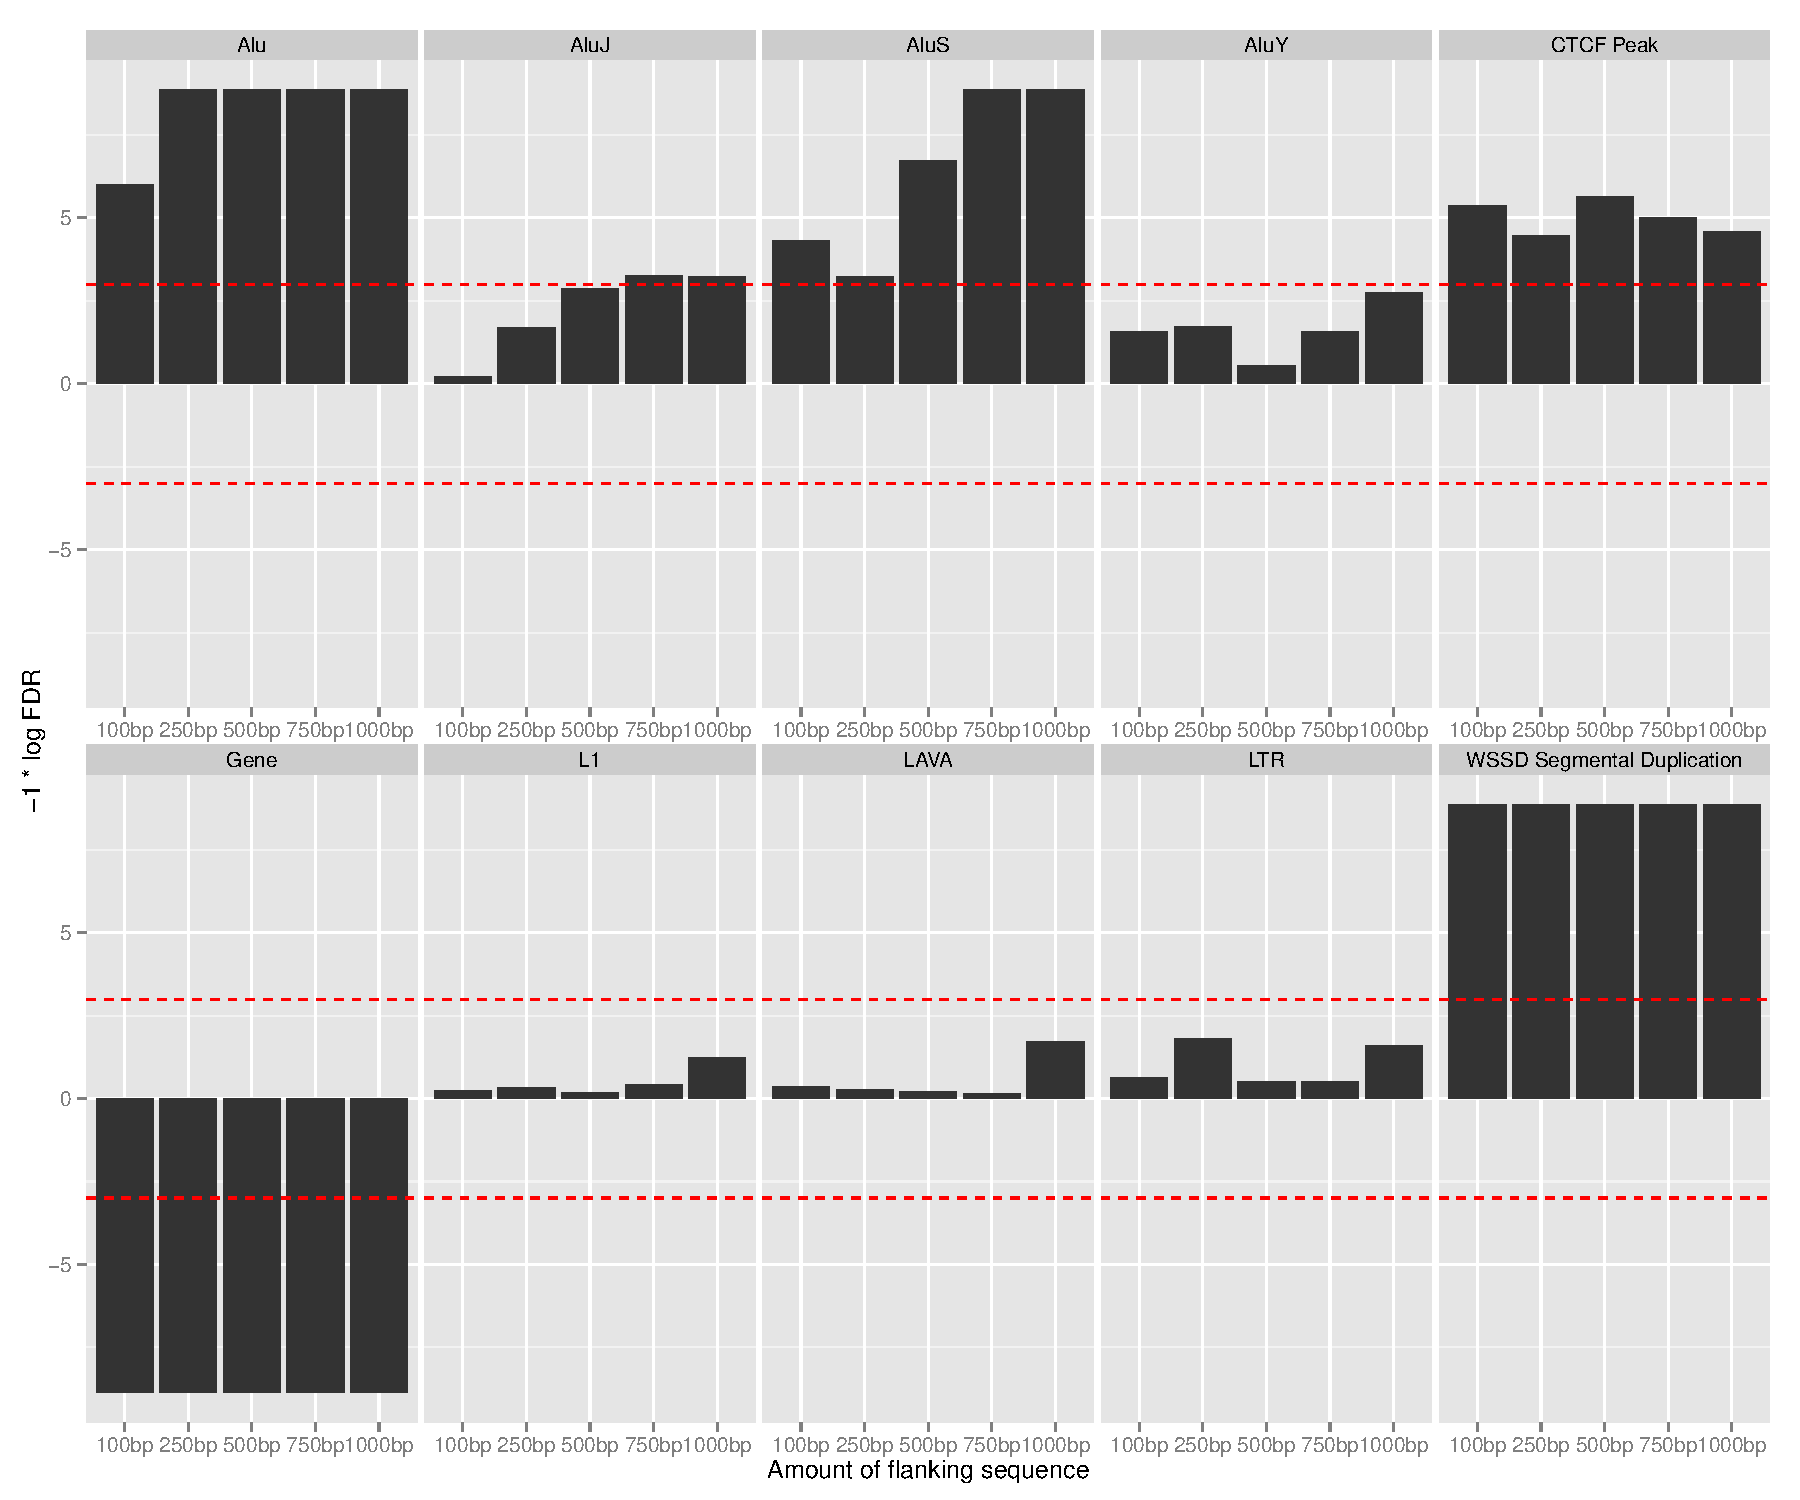
\includegraphics[width=1\textwidth]{figures/regionHitQuantiles.pdf}
\caption{Enrichment or depletion of regions of the gibbon genome for various features, broken down by distance from the breakpoint. Positive y values are the negative log q-values of enrichment for each feature in the regions flanking the breakpoint of the size indicated on the x-axis. Negative y-values represent the q-values of depletion. Q values were calculated using the FDR correction under dependency procedure. The dotted line indicates an FDR threshold of 0.05. Breakpoints are enriched for \emph{Alu} elements, and particularly the \emph{AluS} subfamily, especially at distances of 750bp and 1000bp from the breakpoints. Breakpoints are also enriched for segmental duplications, depleted for genes, and enriched for CTCF binding sites (see Section~\ref{gibbon_ctcf_binding_sites}.)}
\label{gibbon_genome_enrich_by_distance}
\end{figure}

\todo{Even though genes were depleted overall, some of the genes overlapping with breakpoints belong to interesting biological categories \todo{(Table ST5.1 )}.}

In conjunction with our collaborator Larry Wilhelm, in addition to testing the count of overlaps between breakpoint flanking regions and repeats, we also conducted a complementary test that examined the distance of each breakpoint to the nearest repeat of a given class. For this test we used only the 44 breakpoints for which we had single nucleotide breakpoint resolution, with no Gibbon-specific repeats directly intersecting the breakpoint. We compared these breakpoint locations to 10,000 randomly selected regions in the nomLeu2 genome. For each random location, we determined the distance to the nearest repeat. We compared the distribution of distances to a repeat from the breakpoints to the distribution of distances to a repeat from the randomly selected positions using a Kolmogorov-Smirnov test. We examined the distance to any repeat, as well as those for \emph{Alu}, LINE, and LTR elements, and finally the \emph{AluJ}, \emph{AluS}, and \emph{AluY} subfamilies. After FDR correction for multiple hypothesis testing, the distance test showed similar results to the overlap test described above, with significant results for the \emph{Alu} family as a whole, and for the \emph{AluJ} and \emph{AluS} subfamilies, indicating that the breakpoints tend to be closer to those repeats than random locations in the genome.

We also conducted a shift analysis similar to that displayed in Figure~\ref{gibbon_bac_permutations}. Breakpoint regions were simultaneously shifted in increments of 25kb, up to a maximum of 1MB in each direction, and the proportion of breakpoint regions that overlap a feature of interest is reported. Shifts show that breakpoints are centered on regions that are depleted in genes but close to regions that contain genes, while the opposite is true for segmental duplications. \emph{Alu} elements are more evenly spread across the shift regions (Figure~\ref{gibbon_genome_feature_shifts}).

\begin{figure}
\centering
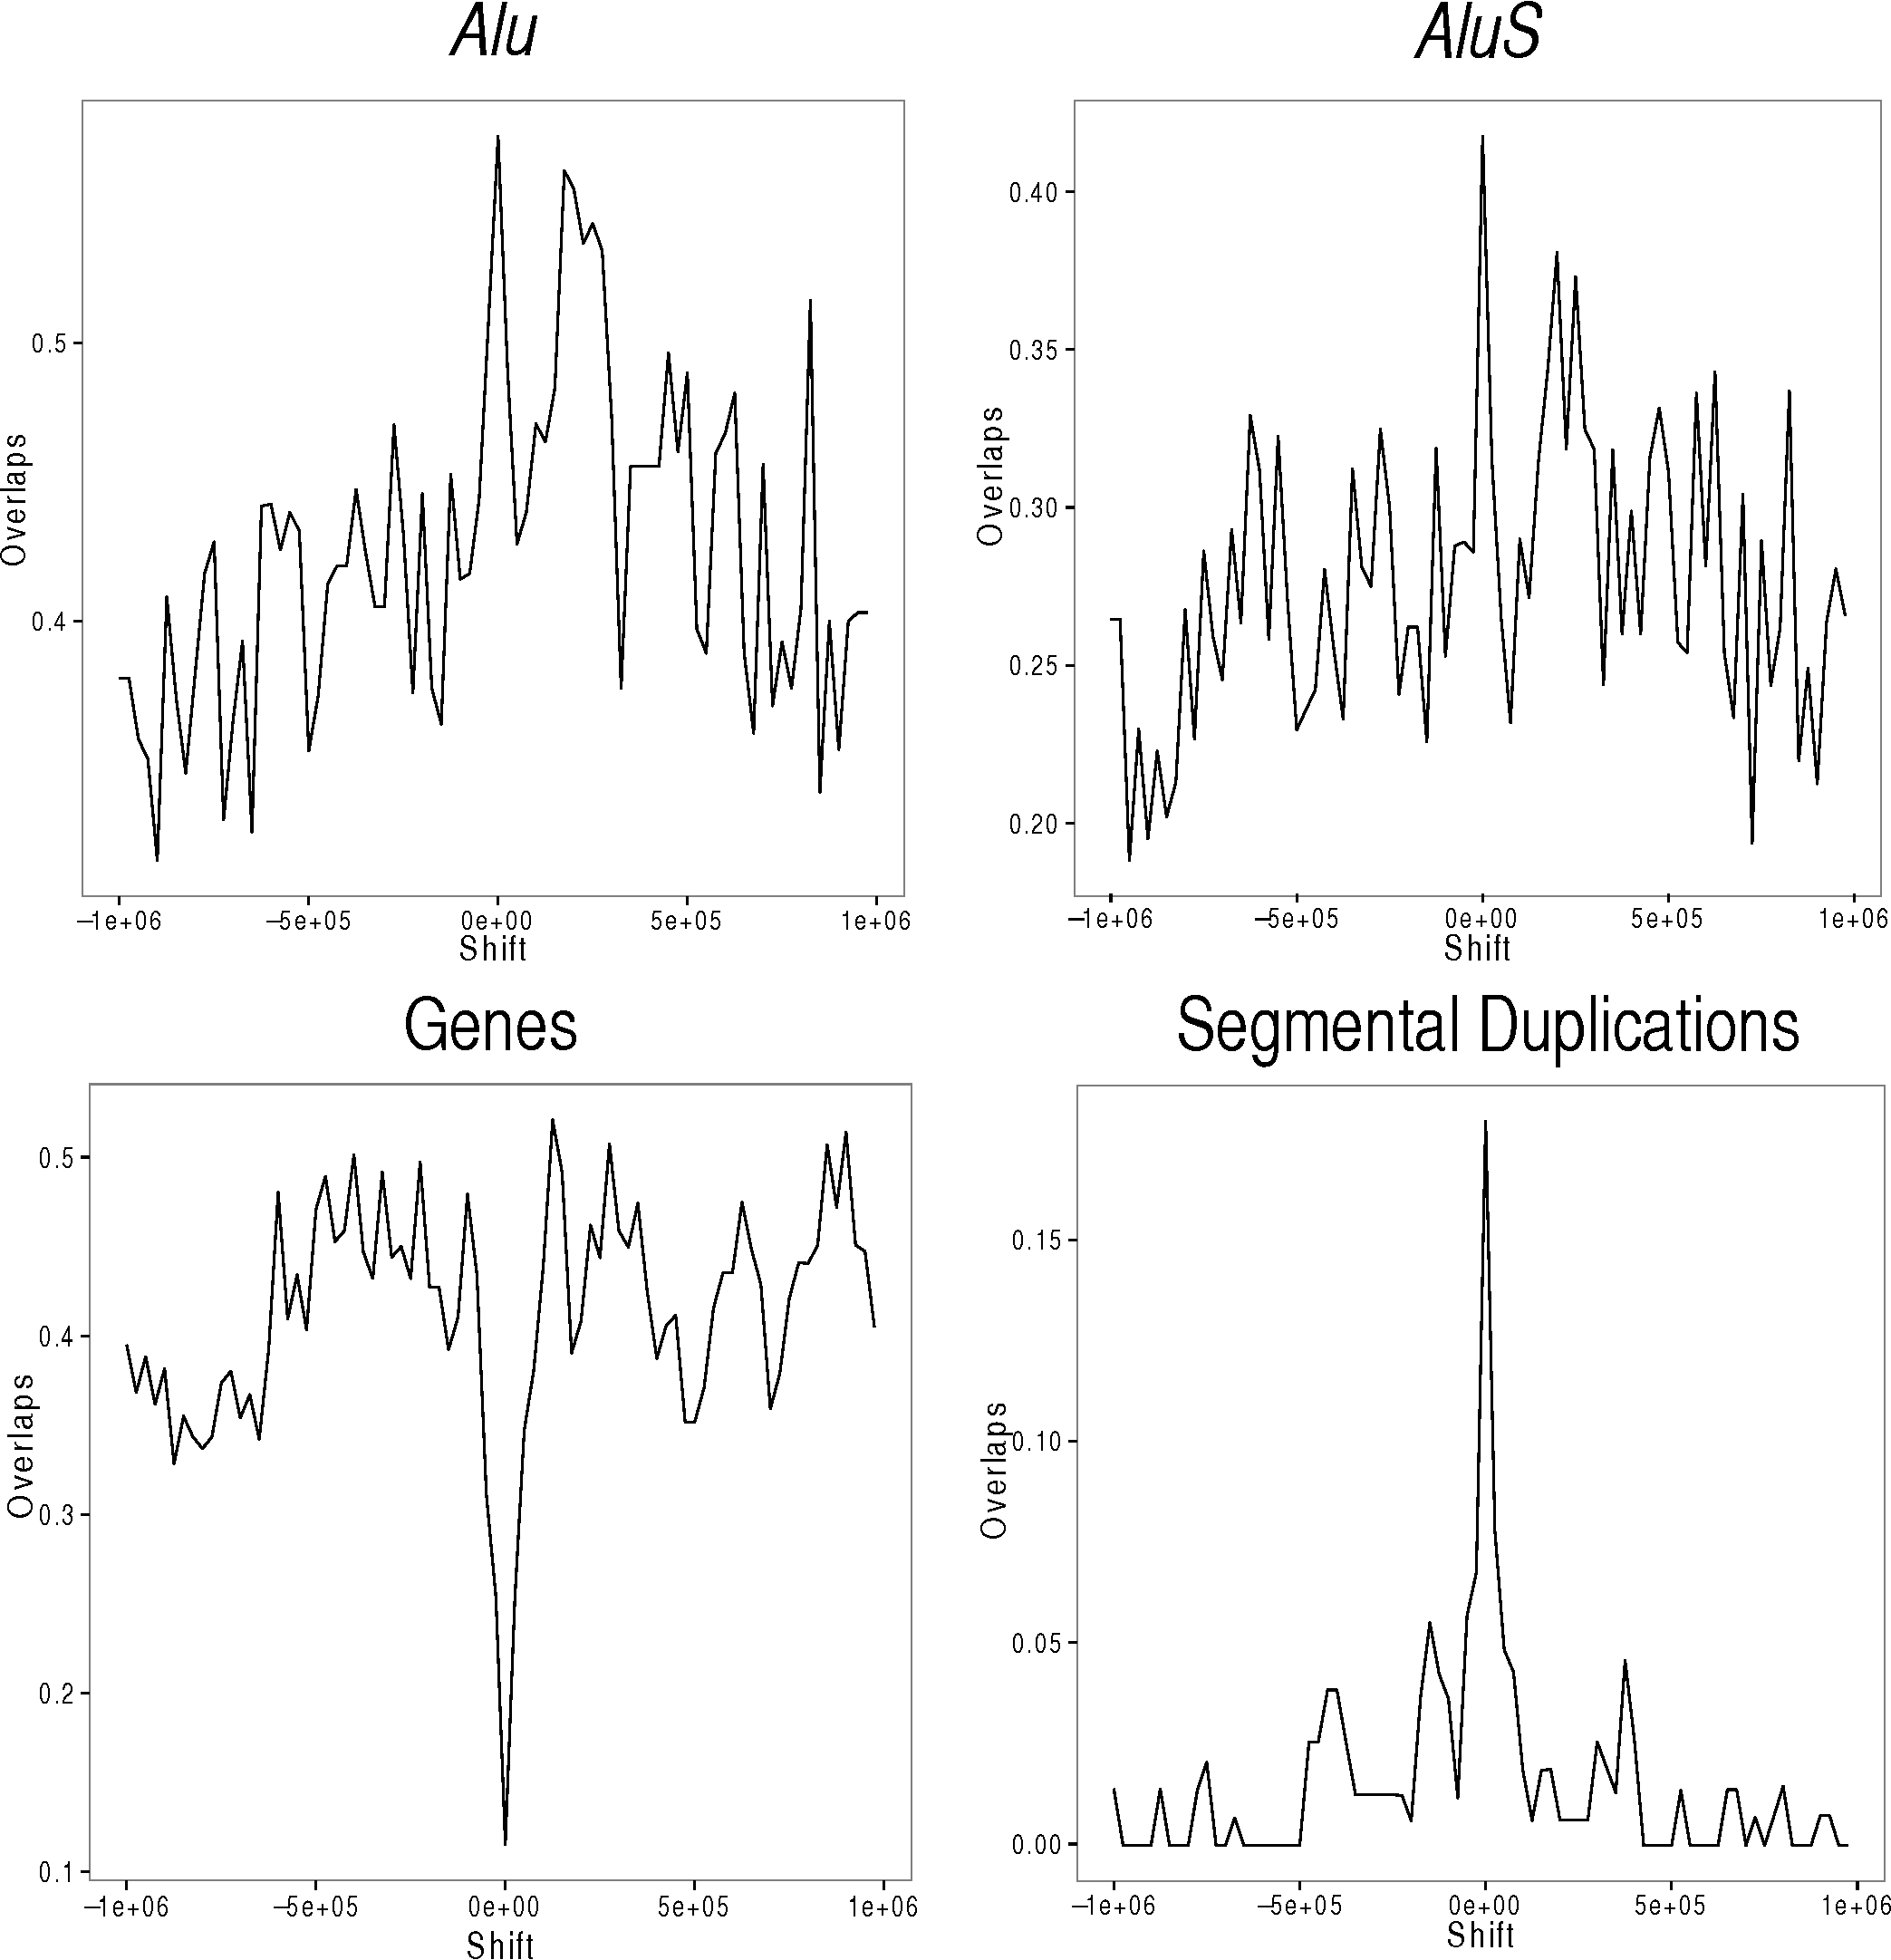
\includegraphics[height=.75\textheight]{figures/gibbon_genome_feature_shifts.pdf}
\caption{The proportion of breakpoint flanking intervals (defined as the 1000bp intervals flanking exact breakpoint locations or gibbon-specific repeats located at the breakpoints) which overlap with a feature of interest, when the flanking intervals are shifted left or right from their actual locations. Breakpoints are located in locations enriched in \emph{Alu} (especially \emph{AluS}) and segmental duplications relative to their genomic neighborhoods, but which are depleted for genes relative to their genomic neighborhoods.}
\label{gibbon_genome_feature_shifts}
\end{figure}

\subsection{Overlap with CTCF Binding Sites}\label{gibbon_ctcf_binding_sites}

Using the gibbon genome reference, we conducted another set of analyses to determine the relationship of gibbon genome breakpoints with binding sites of the evolutionarily conserved binding factor CTCF. CTCF is a transcription factor with many functions, including the ability to separate regulatory domains in the genome from one another~\cite{Phillips:2009fr}. CTCF has also recently been shown to be associated with the three-dimensional structure of DNA and chromatin in the cell~\cite{Dixon:2012gc}, and therefore may have important associations with genomic DNA breakpoints and structural variations. We examined CTCF in the gibbon through the analysis of chromatin immunoprecipitation followed by sequencing (ChIP-seq) data~\cite{Park:2009gl}. Briefly, in ChIP-seq DNA from a sample is cross-linked \emph{in vivo} and then fragmented, so that proteins (in particular transcription factors) remain bound to the fragments of DNA that contain their binding sites. After selecting only those fragments with a bound protein of interest using immunoprecipitation, the DNA is then sequenced. Mapping the reads back to the genome reference sequence creates ``peaks'' of coverage along the genome that indicate the location of transcription factor binding sites. In this analysis we identified a set of CTCF binding sites using gibbon ChIP-seq data, and conducted a comparative analysis using CTCF peaks from other primate species to separate CTCF peaks shared with a common ancestor from those that are unique to gibbons.

\subsubsection{ChIP-seq for CTCF}

CTCF ChIP-seq assays were performed by our collaborators in the laboratories of Duncan Odom and Paul Flicek according to the protocols described in Schmidt et al.~\cite{Schmidt:2012dt} on eight EBV-transformed gibbon lymphoblastoid cell lines. In brief, CTCF-bound DNA was immunoprecipitated using an Anti-CTCF rabbit polyclonal antibody (07-729, Millipore). End-repair was performed on immunoprecipitated and input DNA prior to A-tailing and ligation to single-end Illumina sequencing adapters. DNA was amplified using Illumina primers 1.1 and 2.1 in an 18-cycle PCR reaction. Gel electrophoresis was used to select 200-300 bp DNA fragments. DNA libraries were sequenced using 36 bp reads on an Illumina Genome Analyser II according to the manufacturer's instructions.

\subsubsection{Peak Calling from CTCF ChIP-seq Data}

We aligned reads to the nomLeu2 reference using BWA (version 0.62)~\cite{Li:2009p836} with default parameters, and removed non-uniquely mapping reads. We then called peaks using CCAT~\cite{Xu:2010fu}, with parameters fragmentSize 100, slidingWindowSize 150, movingStep 10, isStrandSensitiveMode 1, minCount 10, minScore 4.0, and bootstrapPass 50. We then combined the peaks called across the different individuals and chose the following set for further analysis: any peak called in an individual individual by CCAT with an FDR of less than 0.05, as well as any peak that was called in more than one individual with an FDR of less than 0.1. \todo{(Table ST5.2)}

\subsubsection{Determination of Gibbon-specific and Shared CTCF Binding Sites}

We classified Gibbon peaks as shared or gibbon-specific by comparing them to a set of CTCF peaks called on human, macaque, and orangutan individuals~\cite{Schwalie:2014}. This work was carried out in conjunction with our collaborators Javier Herrero and Larry Wilhelm. First, orthologous locations of gibbon CTCF peaks in other primate species were determined using a local installation of the EnsemblCompara multi-species alignment database~\cite{ensembl_compara,Vilella:2009ju}. This database contains alignments of the references for human (GRCh37), chimp (CHIMP2.1.4), gorilla (gorGor3.1), orangutan (PPYG2), rhesus macaque (MMUL\_1), and gibbon (Nleu1.1). Gibbon CTCF peaks for which no multi-species alignment were present, or where the nucleotide alignment identity to human and macaque was less than 70\%, were excluded from analysis. We then created a non-redundant list of non-gibbon CTCF peaks by converting the human, orangutan and macaque peaks to gibbon coordinates using the Compara database and removing redundant entries. Shared and gibbon-specific CTCF peaks were then identified as those gibbon CTCF peaks that did or did not intersect a peak in the non-redundant list of non-gibbon CTCF peaks.

\subsubsection{Analysis of Enrichment for CTCF Binding Sites in Gibbon Genome Breakpoints}

We identified 52,685 gibbon CTCF binding sites from the eight individuals. We found that 12 of the 1kb regions flanking breakpoints overlap with CTCF binding sites (see Figure~\ref{example_ctcf_breakpoint} for an example). Using the same permutation analysis described above, this overlap has an enrichment p-value of 0.0009. This effect was even stronger when we expanded the breakpoint flanking regions to 25kb, as 95 expanded flanking regions overlap CTCF peaks for an enrichment p-value <0.0001\todo{(Extended data figure 2)}.

\begin{sidewaysfigure}
\centering
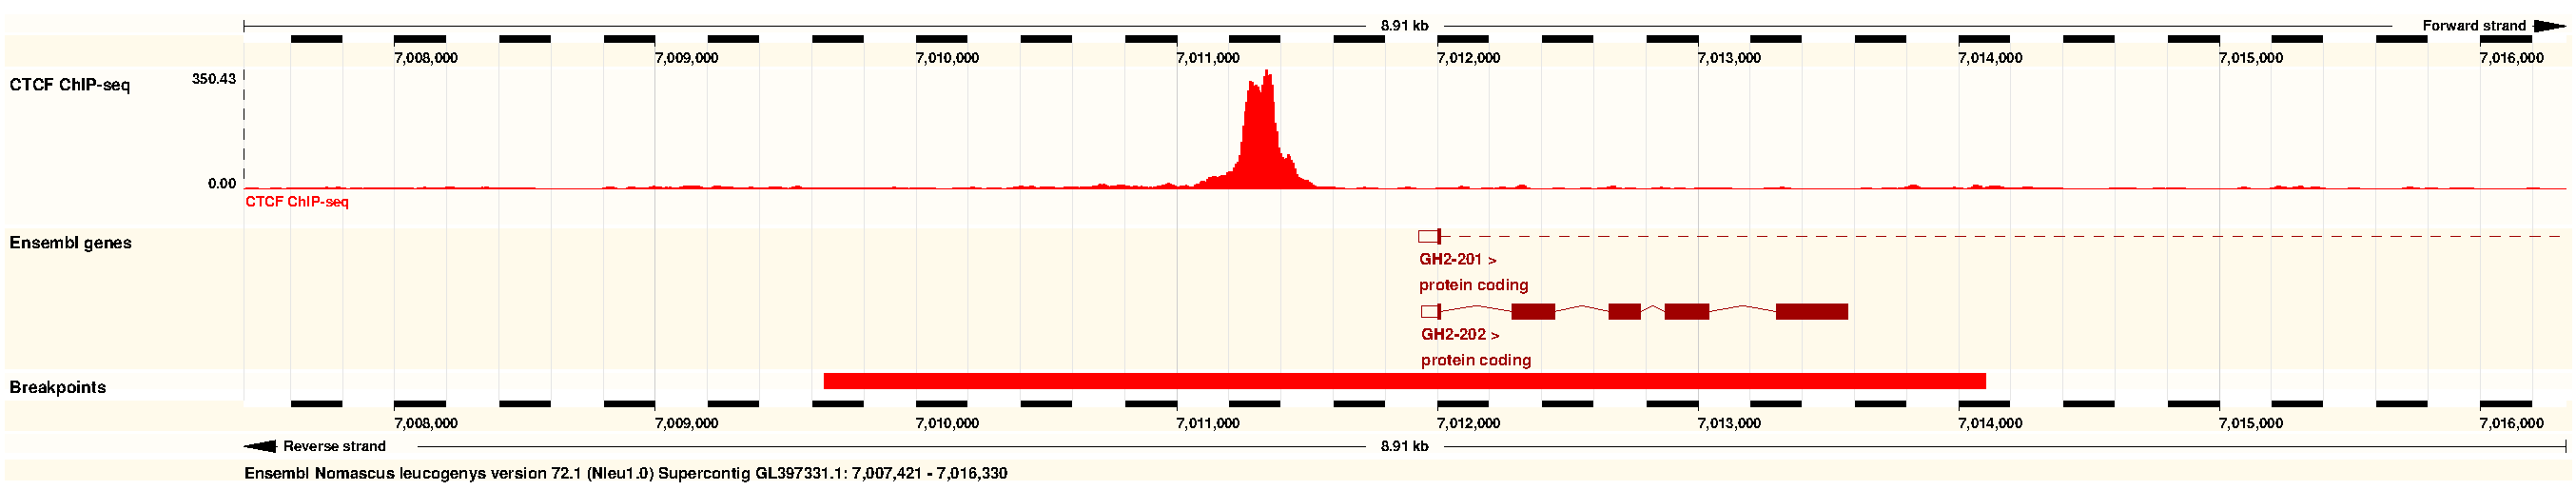
\includegraphics[width=1\textwidth]{figures/merged_CTCF_GL397331.pdf}
\caption{An example of CTCF binding sites in a breakpoint region. The track labeled ``CTCF ChIP-seq'' shows merged read coverage depth from the eight gibbon CTCF ChIP-seq samples, clearly showing a peak representing a CTCF binding site. The ``Breakpoints'' track shows the location of a gibbon breakpoint region. This breakpoint also contains a protein-coding gene, GH2-202.}
\label{example_ctcf_breakpoint}
\end{sidewaysfigure}

We then tested whether the CTCF peaks causing the enrichment in breakpoint regions are specific to gibbons. Using the CTCF ChIP-seq data from other species described above, we classified CTCF binding sites as unique to gibbons (11,449 sites) or shared with a primate ancestor (41,236 sites). We found that the gibbon breakpoint regions are heavily enriched for CTCF binding sites shared with a primate ancestor (enrichment p-value = 0.0006) but are not significantly enriched for gibbon-specific CTCF binding sites. Again, the enrichment is stronger in the 25kb expanded breakpoint regions (enrichment p-value <0.0001) for shared binding sites, but not for gibbon-specific binding sites. This suggests that the formation or selection of gibbon genome rearrangements was associated with ancestral CTCF binding sites.

\todo{I am also helping to analyze the breakpoints from a set of over forty mesenchymal tumor samples in which genomic rearrangements have created ring-shaped chromosomes. The breakpoints that cause these chromosomal rearrangements cluster into several frequently broken areas. I am currently working on analyzing these breakpoint regions using my permutation analysis pipeline in order to determine genomic features that may be significantly associated with these breakpoints, including repeat elements, open chromatin sites and other data from ENCODE, and binding motifs for enzymes known to be involved with breakpoint formation.}

\section{Discussion}

In our work examining breakpoints that included data from HLE and SSY gibbons, we extended previous analyses that had only considered data from NLE. This confirmed that the associations between breakpoints and segmental duplications, genes, and repetitive elements of the \emph{Alu} family previously observed in NLE extended to breakpoints in other genera of the gibbon family. Extending this analysis to the other genera should assist the study of gibbon chromosome evolution, especially when used in conjunction with the release of the gibbon genome reference, which is based on data from an NLE individual.

In Capozzi et al.\cite{Capozzi:2012bb}, we were surprised to find an association between breakpoints and genes given that most genome breaks will have deleterious effects if they occur in coding or regulatory sequence. However, we noted that those results were based on analyzing the features of the human genome reference that are orthologous to the gibbon breakpoint regions, and that the result might change when the full gibbon genome sequence was available to be tested. Indeed, that proved to be the case, as the depletion for genes in the breakpoints from the gibbon reference data shows. This could be an interesting finding in itself, as regions of segmental duplication, which are enriched according to both data sets, are progenitors of novel genes and gene families~\cite{Bailey:2006fn}, possibly providing an explanation for the presence of genes in the orthologous human breakpoint regions.

Our discovery that gibbon genome breakpoints are enriched for CTCF binding sites indicates that there is a connection between regions with similar regulatory environments and the genome rearrangements preserved in the gibbon family, and the fact that breakpoints are only enriched for CTCF binding sites shared with gibbon's common ancestors suggests that the heavy rearrangement of the gibbon genome may have had to respect existing regulatory domains; breakages in other locations may have been too deleterious to survival to be preserved through evolution. In addition, the interaction between genomic structural variation and the three-dimensional structure of DNA in the cell is just beginning to be explored~\cite{Dixon:2012gc}, but it is interesting to hypothesize that locations where the three-dimensional conformation of chromatin in the cell change, as represented by CTCF binding sites, might be vulnerable to genomic breakage under certain circumstances that may have been present in the gibbon's evolutionary past.